\clearpage{\pagestyle{empty}\cleardoublepage}
\chapter{Terzo capitolo}                %crea il capitolo
%%%%%%%%%%%%%%%%%%%%%%%%%%%%%%%%%%%%%%%%%imposta l'intestazione di pagina

\lstloadlanguages{Python}
\lstset{
  language=Python,
  basicstyle=\scriptsize\sffamily,
  numberstyle=\color{gray},
  stringstyle=\color[HTML]{933797},
  commentstyle=\color[HTML]{228B22}\sffamily,
  emph={[2]from,import,pass,return}, emphstyle={[2]\color[HTML]{DD52F0}},
  emph={[3]range}, emphstyle={[3]\color[HTML]{D17032}},
  emph={[4]for,in,def}, emphstyle={[4]\color{blue}},
  showstringspaces=false,
  breaklines=true,
  prebreak=\mbox{{\color{gray}\tiny$\searrow$}},
  numbers=left,
  xleftmargin=-25pt,
  xrightmargin=-50pt,
}

Questo \`e il terzo capitolo.

\section{Creazione del suono}
\subsection{Generazione Sub Bass}                 %crea la sezione
La traccia di sub-bass viene generata tramite un procedimento procedurale implementato nei file sub e wave buffer.
L'unico parametro di cui il processo ha bisogno è l'array di dati relativi alle varie rilevazioni, l'oggetto prodotto è un array di campioni audio stereo.
\subsubsection{Scopo della traccia}
L'aggiunta della traccia di sub bass mira ad aggiungere spessore alla sonificazione durante le rilevazioni particolarmente negative.
Questa traccia è composta da frequenze molto basse, difficilmente udibili se non negli intervalli di condizioni atmosferiche critiche.
Al fine di non rendere la traccia monotona, per ogni intervallo di AQI non ottimale viene sintetizzato un suono diverso.
\subsubsection{Suddivisione dei dati in intervalli}
Il primo passo che questo sottosistema svolge è quello di dividere tutte le rilevazioni in sottointervalli di AQI consecutivi non ottimali.
Per ogni sottointervallo, ne viene indicato l'indice di inizio e quello di fine.
\subsubsection{Generazione delle WaveTable}
In seguito alla suddivisione, per ogni intervallo viene generata una WaveTable.
Per prima cosa viene prelevato il sub-array di dati relativo all'intervallo, in segutio, tramite la classe specificata in wavebuffer.py, viene creato l'array di campioni wavetable.
Partendo dai dati grezzi, ovvero le sole rilevazioni aqi, il primo passo che la classe svolge è quello di aggiungere all'array una sua copia negativa, in modo da rispettare l'ampiezza massima e minima di un segnale audio.
In seguito vengono aggiunti, tramite interpolazione periodica, tanti punti quanti sono i campioni che la WaveTable deve contenere, nel mio caso, 8192.
Ho scelto l'interpolazione periodica per fare combaciare sempre il primo campione con l'ultimo, rendendo l'onda effettivamente periodica.
A seguito dell'interpolazione, ogni campione viene attenuato, ogni valore nella wavetable viene quindi mappato in un valore compreso tra 1 e -1.
Infine, al segnale viene applicato un filtro "Sample n Hold": un circuito che, preso come input un segnale, ne diminuisce la frequenza di campionamento.
L'intervallo di campionamento per il Sample n Hold è stabilito dall'AQI medio, più è alto, più l'onda perde di segnale e risulta invasiva.
\begin{figure}[h]
  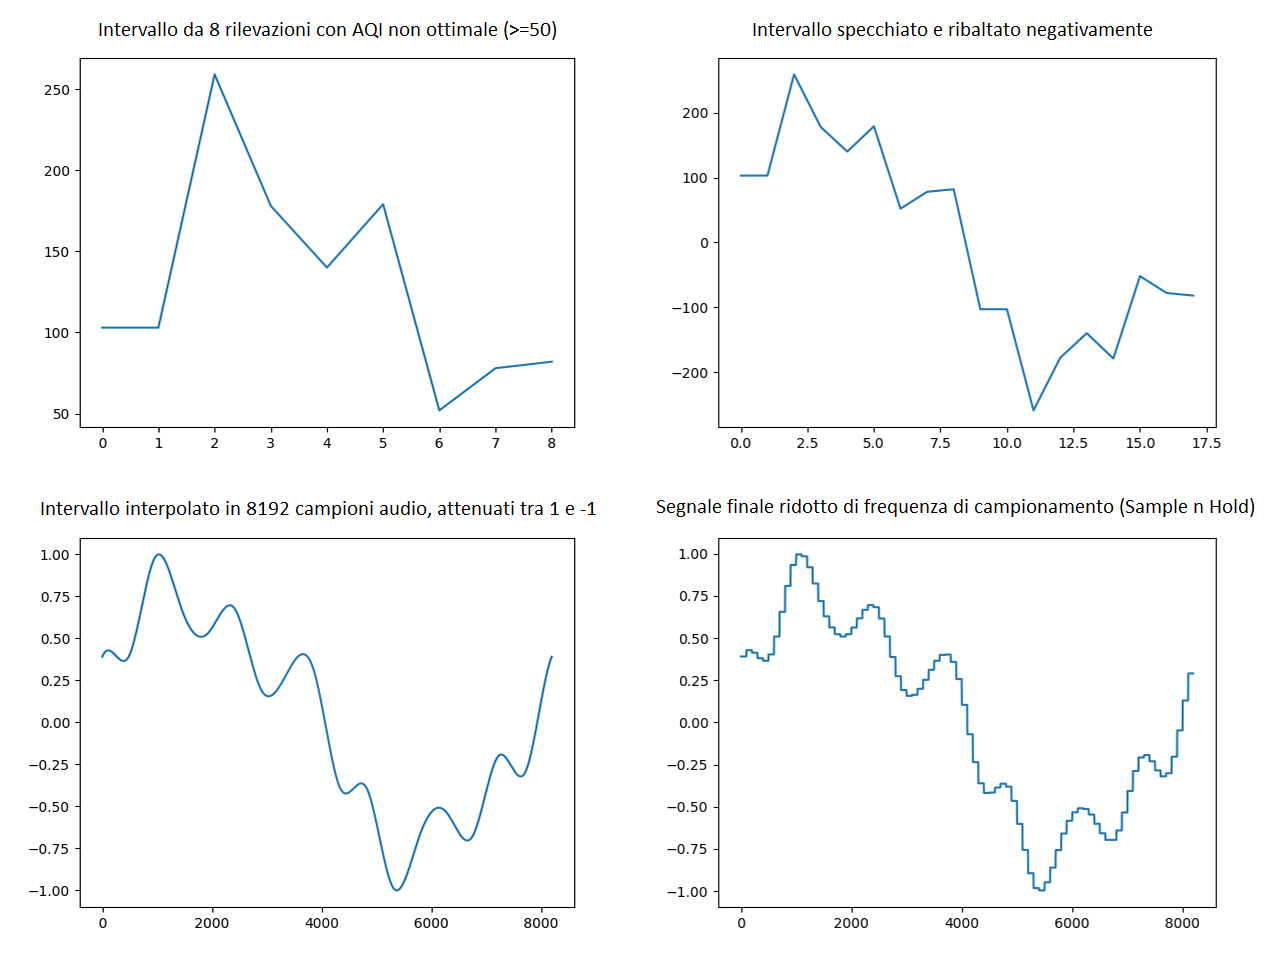
\includegraphics[width=\linewidth]{img/waves.png}
  \caption{Le fasi della generazione di una WaveTable.}
  \label{fig:wavetable}
\end{figure}


\subsubsection{Preparazione dei modificatori di volume - LFO}
Prima di passare alla sintesi vera e propria, il sottosistema definisce gli elementi necessari per l'andamento dinamico del volume.
L'unico elemento utilizzato è l'LFO.
In questa sonificazione, l'LFO appare come una funzione sinusoidale che varia tra 0.5 e 1.5, i valori che andranno a moltiplicarsi al volume.
L'LFO viene creato restituito da una funzione sotto forma di lambda.
\lstset{caption={Generazione dell'LFO.}}
\begin{lstlisting}[language=Python]
def compute_LFO(min, max, samp_period): 
    # samp_period = distanza in campioni tra i picchi della funzione
    freq = 1 / (samp_period / SAMPLE_RATE)
    period = SAMPLE_RATE / freq
    half = (max - min) / 2
    return lambda x: math.sin(2.0 * math.pi * (x) / period) * half + half + min
\end{lstlisting}

\subsubsection{Sintesi}
Ora che tutte le componenti sono pronte, si può passare alla sintesi dell'audio.
La prima cosa che la funzione fa è definire le metriche della traccia, quali il tempo, il numero di note per intervallo, la frequenza di campionamento e la tonalità che si vuole rappresentare.
Per ogni intervallo viene generato un buffer audio, questi verranno poi concatenati in un unico array.
Ogni intervallo è composto da più rilevazioni, ognuna delle quali verrà sonificata con quattro note; il volume e la durata di ogni nota è definita dalla gravità dell'aqi della rilevazione.
I campioni inseriti nel buffer vengono presi dalla WaveTable relativa all'intervallo.
Siccome una WaveTable è composta da abbastanza campioni per suonare ogni frequenza udibile dall'orecchio umano, per rappresentare una certa tonalità, questi vengono selezionati in base alla frequenza di questa.
Il valore di ogni campione viene moltiplicato per il volume, e dalla funzione LFO.
Al fine nascondere le discontinuità delle onde nelle note suonate, ai buffer di ogni nota viene processato da una fuzione "enveloper", che attenua i primi e gli ultimi campioni.

\lstset{caption={Generazione del buffer relativo ad una nota.}}
\begin{lstlisting}[language=Python]
# dur = durata della nota
# step = intervallo di selezione dei campioni per suonare una tonalita
# lfo_ptr = indice globale utilizzato per l'LFO, in modo da non creare oscillazioni di volume discontinue
note_buff = np.array([wavetable[math.floor(i * STEP) % WAVETABLE_SIZE] * vol * LFO(i + lfo_ptr) for i in range(dur)])
\end{lstlisting}



\subsection{Esportare una traccia audio}
L'esportazione e la sintesi delle traccie audio non sintetizzate avviene tramite la classe AudioExporter.
La classe prende come parametri di costruzione le metriche di pentagramma per la traccia, quali il bpm e la suddivisione del tempo.
La funzione di classe volta alla sintesi vera e propria accetta come argomenti una lista di note, un nome per la traccia, l'indice di uno strumento General MIDI e una lista di effetti audio VST3 da applicare.
Le note sono delle strutture dati che contengono le informazioni necessarie per descrivere una nota, sono così composte:
\lstset{caption={Composizione di una nota.}}
\begin{lstlisting}[language=Python]
note = {"note": 44,           # indice della nota
        "time": start_time,   # il tempo di inizio, in battiti 
        "duration": duration, # la durata, in quarti di battito
        "volume": vol}        # il volume 0 - 100, valore facoltativo
\end{lstlisting}
A partire da una lista di note, viene generato un file MIDI .mid, questo viene sintetizzato un un file .wav da timidity++, tramite una chiamata di sistema.
In seguito, il file sintetizzato viene caricato sotto forma di array di campioni stereo, al quale vengono applicati gli effetti audio.
\\
Una volta pronti gli array di tutte le traccie audio, questi vengono uniti in un'unica lista, che viene salvata su un file .wav.
Pevitare errori, ad ogni array viene aggiunto un padding di tanti campioni nulli per rendere tutti gli array della stessa lunghezza.
\lstset{caption={Aggiunta del padding.}}
\begin{lstlisting}[language=Python]
def merge_and_save(*tracks):
  # find max number of samples of track with max num of samples
  # then add padding and merge by sum
  maxlen  = max([len(track[1]) for track in tracks])
  padded  = [np.pad(track, ((0,0), (0, maxlen - len(track[0]))), 'constant', constant_values=0) for track in tracks]
  final   = np.sum(padded, axis=0)
\end{lstlisting}


\subsection{Traccia principale e accordi - Lead}
La traccia principale volte a sonificare l'indice di qualità dell'aria.
Questa traccia si basa su una scala maggiore ed è composta da una nota per rilevazione, presenta un timbro dolce.
La traccia è principalemente presente negli istanti nei quali la qualità dell'aria è ottimale, quando questa peggiora,
il suo volume tende ad abbassarsi lasciando spazio alla traccia di residuo.
Ogni nota è caratterizzata da una tonalità ed un volume che dipendono dalla gravità dell'aqi rispetto al valore maggiore e minore registrato.
Alle note del Lead vengono affiancati degli accordi ripetuti ad ogni battuta, l'ottava di ognuno di questi è determinata dalla media di quattro rilevazioni consecutive.
\lstset{caption={Generazione della traccia principale.}}
\begin{lstlisting}[language=Python]
def get_lead(data, voicing):

  voicing = voicing[::-1]
  n_notes = len(voicing)
  best    = min(data)
  worst   = max(data)
  notes   = []

  for i in range(len(data)):
      aqi       = data[i]
      vol       = 75 if aqi < MIN_THRESH else map_value_int(aqi, best, worst, 50, 25)
      note_idx  = map_value_int(aqi, best, worst, 0, n_notes - 1)
      notes.append({"note": voicing[note_idx], "time": i, "duration": 1, "volume": vol })

  return notes
\end{lstlisting}








\subsection{Creazione del residuo}
Il procsso relativo alla creazione della traccia di residuo è implementato nel file residue.py.
La funzione prende come parametro l'array di rilevazioni AQI, e restituisce una lista di note MIDI.
\subsubsection{Individuare i picchi di residuo}
La prima cosa svolta in questo procedimento è individuare l'andamento del residuo.
Per raggiungere questo scopo, all'array di rilevazioni viene affiancato un array di residuo riempito con il seguente criterio:
Quando viene rilevato un valore AQI non ottimale, il residuo raggiunge tale valore, altrimenti, il residuo viene diminuito di un valore costante.
\subsubsection{Generazione delle note}
Le note sono generate in base agli intervalli di crescita e diminuzione del residuo.
La sonificazione segue questo criterio: appena viene rilevata una fase di crescita, viene creato un arpeggio di note di tonalità ascendenti, che si protrae fino alla fine dell'intervallo.
La frequenza è di quattro note per rilevazione, e le tonalità sono uniformemente distribuite tra le note della scala selezionata; il volume è ascendente.
Alla fase di crescita segue un'eventuale fase di diminuzione, caratterizzata da un arpeggio di note di tonalità e volume discendenti con frequenza di due note a rilevazione. La fase
di discesa si protrae fino alla completa risanazione dell'aria o fino all'inizio di un nuovo intervallo di crescita.
Tramite questa strategia, sono riuscito a differenziare gli arpeggi tra le crescite improvvise di inquinamento e quelle più progressive.
Durante le fasi di crescita e diminuzione del residuo, sono posizionate delle dissonanze in base al valore del residuo.
\begin{figure}[h]
  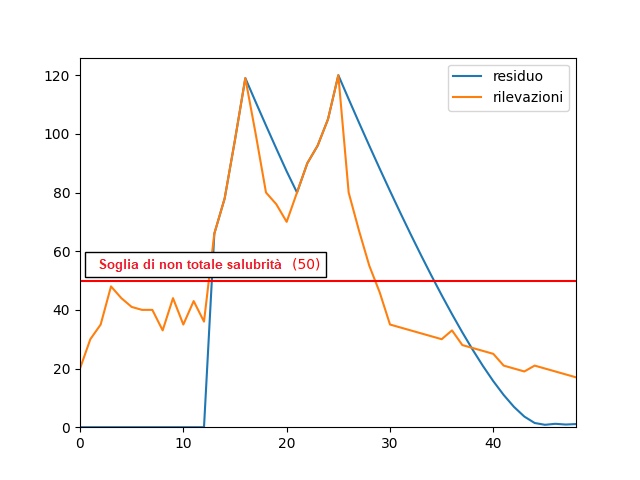
\includegraphics[width=\linewidth]{img/residue.png}
  \caption{L'andamento del residuo con delle possibili rilevazioni.  TODO FIX SALIBRITA'}
  \label{fig:residue}
\end{figure}

